\documentclass[a4paper, oneside]{discothesis}

\usepackage[english]{babel}
\usepackage[utf8]{inputenc}
\usepackage[T1]{fontenc}
\usepackage{algorithm}
\usepackage[noend]{algpseudocode}
\usepackage{hyperref}

%%%%%%%%%%%%%%%%%%%%%%%%%%%%%%%%%%%%%%%%%%%%%%%%%%%%%%%%%%%%%%%%%%%%%%%%%%%%%%%%%%%%%%%%%%%%%%%%%
% DOCUMENT METADATA

\thesistype{Semester Thesis} % Master's Thesis, Bachelor's Thesis, Semester Thesis, Group Project
\title{Simulating Bitcoin's Network Topology}

\author{Lukas Bieri}
\email{lubieri@ethz.ch}

\institute{Distributed Computing Group \\[2pt]
Computer Engineering and Networks Laboratory \\[2pt]
ETH Zürich}

% Optionally, you can put in your own logo here
%\logo{
\includegraphics[width=0.2\columnwidth]{figures/disco_logo_faded}}

\supervisors{Georgia Avarikioti, Roland Schmid\\[2pt] Prof.\ Dr.\ Roger Wattenhofer}

% Optionally, keywords and categories of the work can be shown (on the Abstract page)
%\keywords{Bitcoin Network Graph Blockchain Simulation}
%\categories{ACM categories go here.}

\date{\today}

%%%%%%%%%%%%%%%%%%%%%%%%%%%%%%%%%%%%%%%%%%%%%%%%%%%%%%%%%%%%%%%%%%%%%%%%%%%%%%%%%%%%%%%%%%%%%%%%%

\begin{document}

\frontmatter % do not remove this line
\maketitle

\cleardoublepage

\begin{abstract}
    Bitcoin relies on a peer-to-peer (p2p) network to spread information in an efficient and fair manner across a distributed network. This underlying network and the mapping of its topology is particularly interesting because it determines how efficient and fair those connections are distributed and how fast information can be spread.
    The topology of the network is defined by the connection strategy of the blockchain.
    
    In this thesis, we analyze the standard bitcoin connection strategy and how it compares to several newly developed connection strategies that have been evaluated. The simulation results indicate that the current implementation of the Bitcoin connection strategy works very reliable and efficient compared to other connection protocols. Additionally, having a few nodes that are highly connected within the network or increasing the number of minimal connections per node on every node from currently 8 to 13 connections indicates a decrease of the length of the shortest paths between nodes.
\end{abstract}

\tableofcontents

\mainmatter % do not remove this line

% Start writing here
\chapter{Introduction}

Bitcoin is a distributed network and relies on a fast and fair information exchange between its nodes to safeguard the security of its transactions. The gossiping between individual nodes is the only way peers get information about the current state of the network. This underlying peer to peer network allows them to agree on new blocks that are mined.

Thus, the minimization of the propagation delay of a new block that is mined is crucial for the whole network. However, the exact topology of the network is intentionally hidden which makes it hard to reason about possible attacks or manipulations that could occur in the Bitcoin network. For example one study has revealed that an ``advantage`` in the Bitcoin networks' broadcasts can be transferred directly into coin gains~\cite{MajorityIsNotEnough}.

This thesis looks at comparing new possible connection strategies versus the current implementation of the Bitcoin network by means of simulation. The simulation is ran on a self-developed simulation tool which is based on the standardized Bitcoin implementation.~\footnote{As part of the project I built a simulation environment from scratch in python to test and compare different network connection strategies and hypotheses. The source code of the simulation can be pulled from Github as open source code. \url{https://github.com/lukebieri/bitcoinTopologySimulation}}
Firstly, a brute-force approach where the number of edges was increased is examined. Such a brute-force approach indicates to be a promising approach to increase speed and fairness.
Secondly, two algorithms were developed where a node that wants to connect to a neighbouring node asks its neighbour for its degree and connects either to the higher or lower number of degree node. Using this approach leads to either more speed and less fairness or less speed and more fairness.
Thirdly, an algorithm was developed where a Bitcoin node differentiates other nodes based on their IP location into different clusters. Using different propagation delays for local versus international connection indicates that such a geographical mapping algorithm does perform similarly to the standard Bitcoin implementation.

Additionally, various degree distributions deviations from the standard Bitcoin protocol are taken into account to achieve more real world behaviour and explore what happens if some nodes deviate from the standard implementation.

\chapter{Background}

Bitcoin runs on decentralized nodes that pass messages purely in a peer-to-peer network to manage electronic cash transactions and has no official administrator as Nakamoto~\cite{SatoshiPaper} initially suggested in his famous paper. Thus, the challenge is to build a network that converges to a global and coherent state while having a fast and robust network topology.
Tschorn et al.~\cite{BitcoinAndBeyond} showed how exactly the standard bitcoin protocol~\cite{GithubBitcoin} with its design choices is developed and discusses the key ideas behind it.

Furthermore, Miller et al.~\cite{DiscoveringBitcoinsPublicTopologyAndInfluentialNodes} developed a method to observe and analyze the Bitcoin network in its current state. The so-called ``AddressProbe`` technique relies on the two hours penalty that is taken into account for received address messages from connected neighbours specified by the Bitcoin protocol to infer this information. Miller et al.~\cite{DiscoveringBitcoinsPublicTopologyAndInfluentialNodes} found that of all nodes there exist some highly connected and influential nodes that connect to many other nodes (range of hundreds) and thus, deviating from the standard implementation of the Bitcoin protocol~\cite{GithubBitcoin}. Thus, the ``AddressProbe`` technique proved that the Bitcoin network is not a random graph. However, after the release of the Bitcoin Core 0.10.1 their ``AddressProbe`` technique does not work anymore~\cite{BlockchainInnefficiency}.

\section{Topology of Bitcoin}
In this section we describe how the current connection strategy of the official Bitcoin implementation is designed. Non-essential details may be omitted for simplicity of the presentation.

\subsection{Joining the Bitcoin Network}
Though, a new node that wants to connect to the Bitcoin network finds their first peers by querying one of Bitcoin's DNS server from a set of hard-coded DNS servers. Through this query it gets a list of Bitcoin nodes and from now on it tries to populate and update this list further. This is done by ``getaddr`` requests~\cite{protocolDocumentation} to other nodes where individual nodes exchange random subsets of their private address lists called ``addr`` messages with requesting nodes.

\subsection{Connecting to Peers}
Each Bitcoin node tries to maintain a minimum number of 8 connections to other nodes within the network. It tries actively to reach these 8 connections by choosing addresses randomly out of its local list of addresses.
However, a node does not accept more than 125 connections to avoid running out of internet bandwidth.

For each locally saved address that has been shared due to a ``getaddr`` call or a connection request there is a timestamp attached to it such that every node is able to remove certain outdated addresses.
All nodes query what information is known by their neighbours every 24 hours to keep the table updated. This makes sure that information about a newly connected node eventually floods the whole network.

In addition, a Bitcoin node tries to hide its active connections from its neighbours and will not reveal all its neighbours in a ``getaddr`` call. Knowing all neighbours of a peer could significantly increase the success probability of a double spending as Nick~\cite{guessingP2P} claims.

\section{Technical Design of the Simulation}
Since a whole Bitcoin network has to be simulated there needs to be an adequate design choice. Running a simulation with a few thousand threads where each thread represents a single Bitcoin node with the code from the official Bitcoin implementation~\cite{GithubBitcoin} would have used up too much computational resources. There would have been a big overhead and the simulation would have been utterly complex regarding code that is not relevant for the outcome of this thesis.

We thus concluded that a new simulation environment had to be built from scratch. For a general overview, one may consult Figure [~\ref{fig:BitcoinSimulationDiagram}] along the following explanation.

All major parameters can be specified in the ``main.py`` file which launches one or multiple python simulations accordingly. There are various parameters that can be set according to the kind of simulation one is interested in. The most important parameters for this thesis are the distribution of the initial nodes a single Bitcoin node wants to connect as well as its limit, the connection protocol and the size of the simulation respectively how many nodes that should be used.
The simulation class in ``simulation.py`` builds a Bitcoin network on a networkx instance~\cite{networkx}. Networkx is a framework provided by the python community for graph representations as well as calculations. It is particularly useful such that it provides algorithms to calculate the shortest path lengths.
Additionally, each node of the graph has an object from the class BitcoinNode in ``bitcoinNode.py``. The class BitcoinNode takes care of the connection strategy of an individual node according to its initialization that are being set in the simulation class. It has locally stored all relevant information that are being used by a real Bitcoin node to take decisions on how it should connect to other nodes and the relevant protocols for doing so. As a result all decisions regarding the opening of new connections to other nodes are being taken by the BitcoinNode class. Thus, the Simulation class just needs to maps the rewiring that have been agreed on by two individual Bitcoin nodes to the networkx data structure. It can do so by observing messages that are passed between individual Bitcoin nodes.
These messages are organized as dictionaries and called ``envelopes``. They play a crucial part because these messages are the only mean of communication for Bitcoin nodes. They are either filled with message data to either give the simulation class feedback about its state or to send a message to another node. Therefore, the Simulation class also acts as a transport layer for individual Bitcoin nodes.

The core of the simulation is written in time intervals such that in every time interval all nodes in the network are asked if they want to request new ``getAddr`` calls, if they have to build new connections or if there are messages from other nodes that need to be handed over to a particular node to get a response.
Additionally, there are two types of nodes. A node can either be a normal Bitcoin node that wants to connect to the network or there is a fixed number of nodes that act as initial DNS nodes that are being requested when a new node wants to connect to the Bitcoin network.

During runtime in predefined time slots and at the end of the simulation the class Simulation calls the class NetworkAnalytics in ``networkAnalytics.py``. The class NetworkAnalytics analyzes the network and plots the result. It does not perform any rewiring on the graph itself and is just used for analytical purposes. Though, in this class the shortest path length function of the networkx library is called. Depending on the number of nodes in the network and the number of edges this can be a  time consuming call lasting from a couple of seconds up to more than an hour depending on the simulation and the hardware available.

\begin{figure}
    \centering
    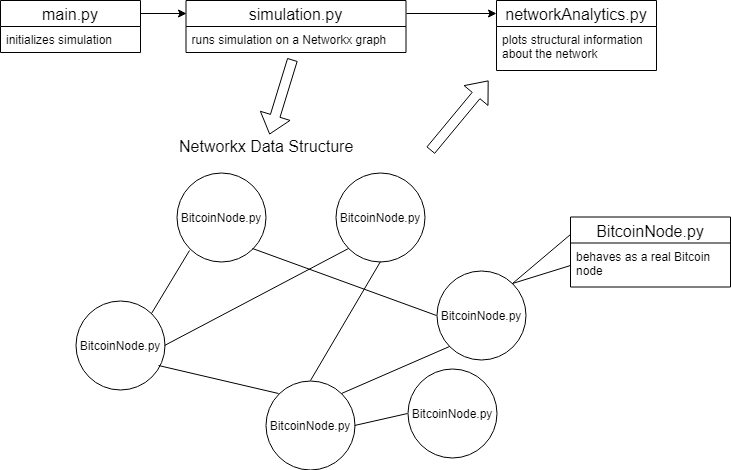
\includegraphics[width=1\columnwidth]{figures/BitcoinSimulationDiagram}
    \caption{The simulation runs on a networkx data structure where each node has a BitcoinNode object stored in it. These BitcoinNode object give a single node the ability to communicate with other nodes to come to common agreements about new connections. The Simulation class therefore acts as transport layers of messages that are being sent between nodes, maps new nodes to the network as well as taking nodes offline and observing messages that are being sent between individual nodes to keep the edges updated with the information that is being exchanged between individual Bitcoin nodes. The networkAnalytics class is called on predefined time intervals and on the end of a simulation to analyze the network by calculating the shortest path lengths inside the network or looking at degrees for example.}
    \label{fig:BitcoinSimulationDiagram}
\end{figure}

\chapter{New Connection Strategies}

In this thesis two main approaches with some variations for a new connection strategy have been chosen to be developed further to set against the standard Bitcoin protocol implementation.

\section{Power of Two Choices}
The power of two choices method describes the following problem. Assume that $n$ balls have to be placed in $n$ bins independently and uniformly at random.

Mitzenmacher et al.~\cite{Power2Choices} have shown that the maximum load (largest number of balls in any bin) is approximately $$\frac{\log n}{\log \log n}.$$
In addition they have shown that if one now adds the additional property that the balls are placed such that they are placed in the least loaded bin of $d \geq 2$ the maximum load is $$\frac{\log \log n}{ \log d} + O(1)$$ with high probability.

One can now apply this powerful idea of the power of two choices method to the Bitcoin connection strategy assuming each node in the network as being a bin and every new node that connects to the network represents a ball.
The idea behind it is to balance the degree distribution evenly between all Bitcoin nodes. This should be achieved if a node that wants to add one connection gets two random addresses from its cache and asks both of those nodes chosen for their degree. Afterwards the node that asked for the degree gets back the two messages and will connect to the node with the lower degree. This algorithm is described in the appendix in more detail [~\ref{alg:power2choicesMin}].
The expectation we get from this protocol is that it takes on average roughly the same number of hops for each node to reach all other nodes due to this degree balancing that we believe leads to a network where each node should be connected to the network equally well.

If one now adapts this powerful idea of the power of two choices method to the bitcoin connection strategy one comes to the following algorithm [~\ref{alg:power2choicesMin}].

Additionally, out of curiosity the algorithm was also slightly modified such that not the node with the minimum degree was chosen to be connected, but instead the node with the maximum degree gets selected as illustrated in algorithm [~\ref{alg:power2choicesMax}].

\begin{algorithm}
\caption{Power of two Choices with the minimum number of nodes selected} \label{alg:power2choicesMin}
\begin{algorithmic}[1]
\Procedure{p2cmin}{$addrMan$} \Comment{$addrMan$ has data}
\While{own degree < 8}
    \State choose addresses $A1$ and $A2$ u.a.r. from $addrMan$
    \State ask $A1$ and $A2$ about their degrees $D1$ and $D2$
    \If{$D1 \geq D2$}
        \State connect to $A2$
    \Else
        \State connect to $A1$
    \EndIf
\EndWhile
\State \textbf{return} \Comment{node is fully connected}
\EndProcedure
\end{algorithmic}
\end{algorithm}

\begin{algorithm}
\caption{Power of two Choices with the maximum number of nodes selected} \label{alg:power2choicesMax}
\begin{algorithmic}[1]
\Procedure{p2cmax}{$addrMan$} \Comment{$addrMan$ has data}
\While{own degree < 8}
    \State choose addresses $A1$ and $A2$ u.a.r. from $addrMan$
    \State ask $A1$ and $A2$ about their degrees $D1$ and $D2$
    \If{$D1 \leq D2$}
        \State connect to $A2$
    \Else
        \State connect to $A1$
    \EndIf
\EndWhile
\State \textbf{return} \Comment{node is fully connected}
\EndProcedure
\end{algorithmic}
\end{algorithm}

\section{IP Location Clustering}
Propagation delays of messages that are being sent between a sender and a receiver correlate with the geographical location of the individual nodes~\cite{geoDelay}.
Using the IP location information could therefore potentially help nodes that want to add a connection to minimize propagation delays. A single node could therefore spread information on average faster to nodes that are localized closer to itself and ideally minimize average path delays. Thus, Bitcoin nodes could be grouped into clusters of geographically nearby nodes. The property of a single cluster would be that it is able to spread information fast within its cluster because of its geographical location but it takes more time to reach other clusters since they are (geographically) far away; therefore have on average a longer propagation delay. 
This would allow a node that wants to send information to all other nodes to firstly pass it to its own cluster. In its own cluster it would spread very quickly among all neighbours of the same cluster. Secondly, it would pass this information to other nodes that are located in different geographical clusters. It would take some time for this message to pass to the other clusters but as soon as they have been reached it will spread very quickly within the clusters further away. Thus, the longest hop (between two clusters) would be made at the beginning and the message could afterwards profit from low latencies expected within geographical clusters that are further away.

The practical implementation of this idea has been done as follows. We defined 6 clusters, namely Europe, South-America, North-America, Asia, Africa and Oceania. 6 clusters have been chosen to give each continent respectively geographical region a similar weight and accounting for fast connections that exist inside continents. Additionally, having 6 clusters leaves every node with 5 other clusters which is a reasonable number if the initial connections of a Bitcoin node is 8. Thus, two different approaches have been analyzed in more detail.
Firstly, there is an approach where one chooses 3 nodes within the same cluster and 1 node from each other cluster as illustrated in algorithm [~\ref{alg:geo3to5}] with 8 initial connections for each node.
Secondly, there is an approach where one chooses 8 nodes within the same cluster and 1 node to each other cluster as illustrated in algorithm [~\ref{alg:geo8to5}] with 13 initial connections for each node.

\begin{algorithm}
\caption{3 local, 5 intercontinental}\label{alg:geo3to5}
\begin{algorithmic}[1]
\Procedure{geoConnection}{$addrMan$} \Comment{$addrMan$ has data}
\While{own degree < 8}
    \State choose address $A1$ u.a.r. from $addrMan$\;
    \State look-up cluster $C1$ from $A1$\;
    \If{no connection exists to $C1$}
        \State connect to $A1$
    \ElsIf{number of connections to own cluster < 3}
        \State connect to $A1$\;
    \EndIf
    \EndWhile
\State \textbf{return} \Comment{node is fully connected}
\EndProcedure
\end{algorithmic}
\end{algorithm}

\begin{algorithm}
\caption{8 local, 5 intercontinental}\label{alg:geo8to5}
\begin{algorithmic}[1]
\Procedure{geoConnection}{$addrMan$} \Comment{$addrMan$ has data}
\While{own degree < 13}
    \State choose address $A1$ u.a.r. from $addrMan$\;
    \State look-up cluster $C1$ from $A1$\;
    \If{no connection exists to $C1$}
        \State connect to $A1$
    \ElsIf{number of connections to own cluster < 8}
        \State connect to $A1$\;
    \EndIf
    \EndWhile
\State \textbf{return} \Comment{node is fully connected}
\EndProcedure
\end{algorithmic}
\end{algorithm}

\chapter{Results}

\section{Standard Bitcoin Implementation}

The results of the standard Bitcoin implementation simulation are shown in Figures [~\ref{fig:standardBitcoinAverageHops},~\ref{fig:standardBitcoinDegree},~\ref{fig:standardBitcoinShortestPaths}]. We observe in Figure [~\ref{fig:standardBitcoinAverageHops}] that the number of average hops peaks at 4 hops and indicates a Gaussian distribution. Looking at the degree distribution of Figure [~\ref{fig:standardBitcoinDegree}] the number of nodes of a particular degree starts at the minimum initial degree number of 8 and peaks at 16 edges (double the initial degree distribution) and decays exponentially afterwards. Since the maximum number of degree is 41 we conclude that there are no rough nodes that try to connect to as many nodes as possible.
Regarding shortest paths between any two nodes within the network as in Figure [~\ref{fig:standardBitcoinShortestPaths}] most of the time it takes 4 hops from one node to any other node. Slightly more nodes can be reached with 3 hops than with 5 hops. Additionally, one usually needs 3, 4 or 5 hops to reach any other node in the network with comparable few pairs that can be reached quicker or that take longer.

\begin{figure}
    \centering
    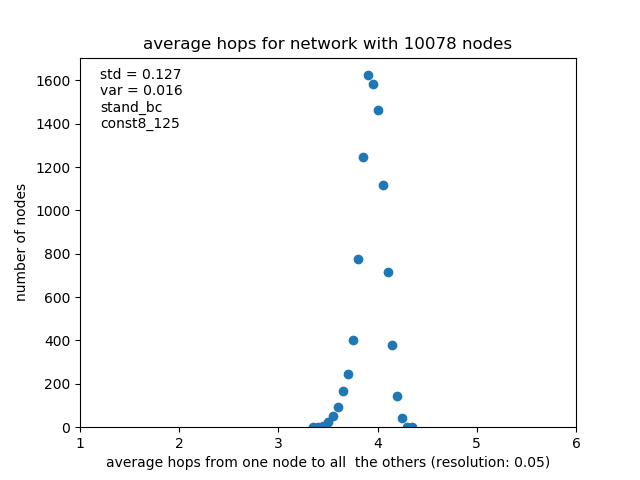
\includegraphics[width=.8\columnwidth]{figures/standard-bitcoin/average-hops-for-network-with-10078-nodes.png}
    \caption{The average path distance from one node to any other nodes using the standard Bitcoin implementation.}
    \label{fig:standardBitcoinAverageHops}
\end{figure}

\begin{figure}
    \centering
    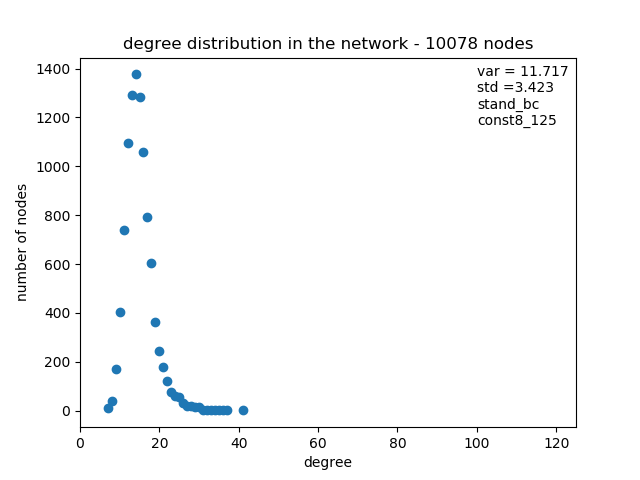
\includegraphics[width=.8\columnwidth]{figures/standard-bitcoin/degree-distribution-10078-nodes.png}
    \caption{The degree distribution from the standard Bitcoin implementation.}
    \label{fig:standardBitcoinDegree}
\end{figure}

\begin{figure}
    \centering
    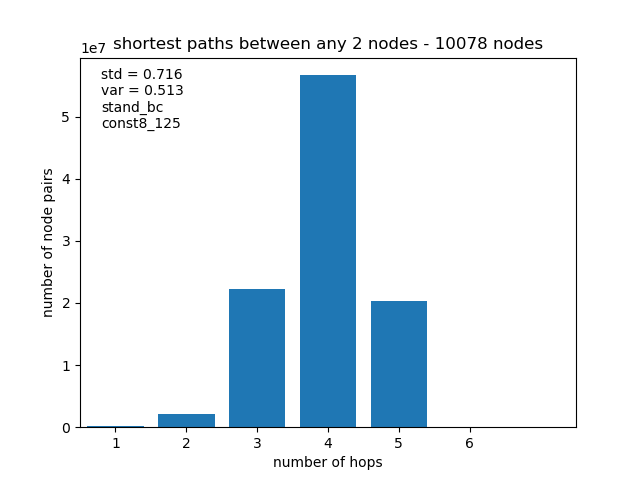
\includegraphics[width=.8\columnwidth]{figures/standard-bitcoin/final-shortest-paths-between-any-nodes-10078-nodes.png}
    \caption{The shortest paths between any two nodes from the standard Bitcoin implementation.}
    \label{fig:standardBitcoinShortestPaths}
\end{figure}

\section{Influence of Initial Connections}

In this subsection we present and analyze the simulation results of varying the number of the initial connections, illustrated in Figures [~\ref{fig:initConnectDistribution8variation-big},~\ref{fig:initConnectDistribution8variation-small}]. In the standard Bitcoin protocol these initial connections are set to 8 for all nodes. For performance reason this simulation was only done with 3000 nodes.
It illustrates clearly that if one increases the number of initial connections the average shortest path increases quite a bit. However, for 3000 nodes at approximately 48 initial connections and more there is a flattening of the curve at an average hop at around 2.5. Simulation shows that the average shortest path between any node can hardly go below that limit with a ``reasonable`` number of initial connections.

\begin{figure}
    \centering
    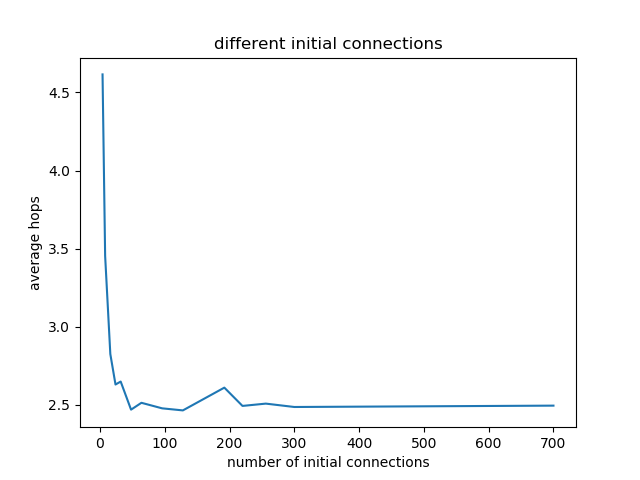
\includegraphics[width=.8\columnwidth]{figures/initConnectDistribution/8variation/3000nodes-bigRange.png}
    \caption{Average of shortest paths between any node using different initial connections in each round of simulation using 3000 nodes.}
    \label{fig:initConnectDistribution8variation-big}
\end{figure}

\begin{figure}
    \centering
    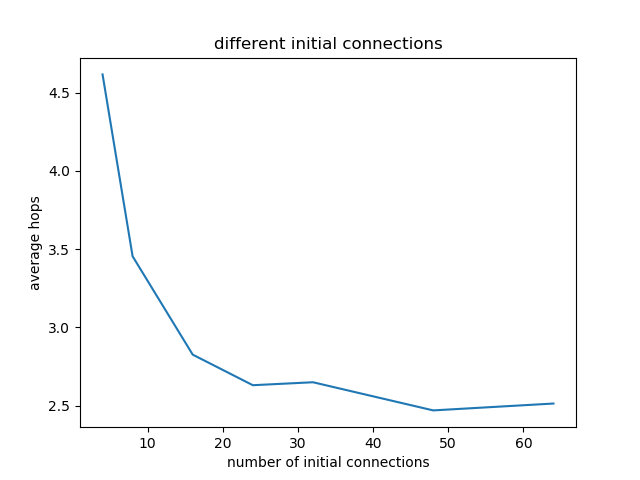
\includegraphics[width=.8\columnwidth]{figures/initConnectDistribution/8variation/3000nodes-smallRange.png}
    \caption{Average of shortest paths between any node using different initial connections in each round of simulation using 3000 nodes. (zoom of [~\ref{fig:initConnectDistribution8variation-big}])}
    \label{fig:initConnectDistribution8variation-small}
\end{figure}

\subsection{13 initial connections}

In this subsection we present the simulation results of having replaced the initial 8 connections with 13, illustrated in Figures [~\ref{fig:initConnectDistributionConst13Average},~\ref{fig:initConnectDistributionConst13Degree},~\ref{fig:initConnectDistributionConst13ShortestPath}].
Looking at the average hops in Figure [~\ref{fig:initConnectDistributionConst13Average}] the peak, the standard deviation and the variance decrease compared to the standard Bitcoin implementation in Figure [~\ref{fig:standardBitcoinAverageHops}]. The nodes inside the network have now much higher degree as illustrated in Figure [~\ref{fig:initConnectDistributionConst13Degree}] and thus there are more edges within the network. Additionally, the shortest paths between any two nodes as illustrated in Figure [~\ref{fig:initConnectDistributionConst13ShortestPath}] decreases as well compared to the standard Bitcoin implementation in Figure [~\ref{fig:standardBitcoinShortestPaths}] and now peaks at 3 hops. However, there are still many node pairs that are only reachable by 4 hops.

\begin{figure}
    \centering
    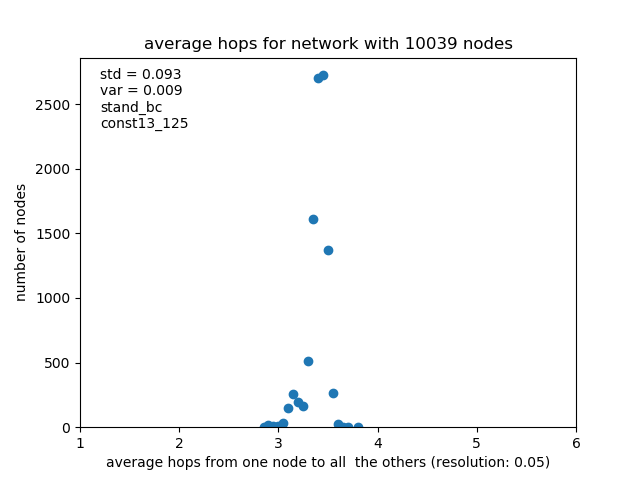
\includegraphics[width=.8\columnwidth]{figures/initConnectDistribution/const13/average-hops-for-network-with-10039-nodes.png}
    \caption{Average hops from one node to all other nodes using the standard Bitcoin implementation with 13 initial connections.}
    \label{fig:initConnectDistributionConst13Average}
\end{figure}

\begin{figure}
    \centering
    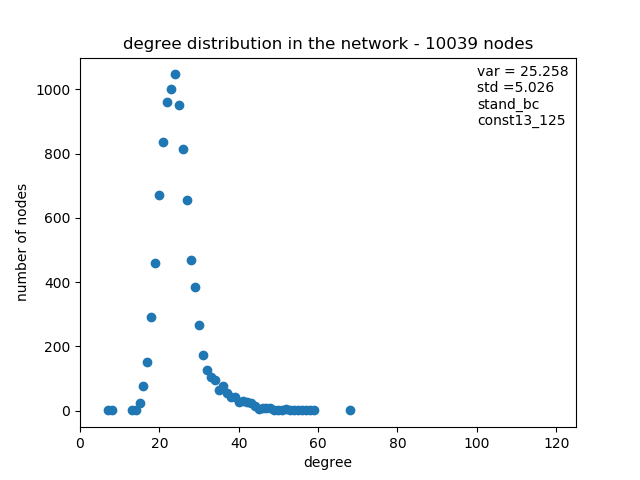
\includegraphics[width=.8\columnwidth]{figures/initConnectDistribution/const13/degree-distribution-10039-nodes.png}
    \caption{Degree distribution using the standard Bitcoin implementation with 13 initial connections.}
    \label{fig:initConnectDistributionConst13Degree}
\end{figure}

\begin{figure}
    \centering
    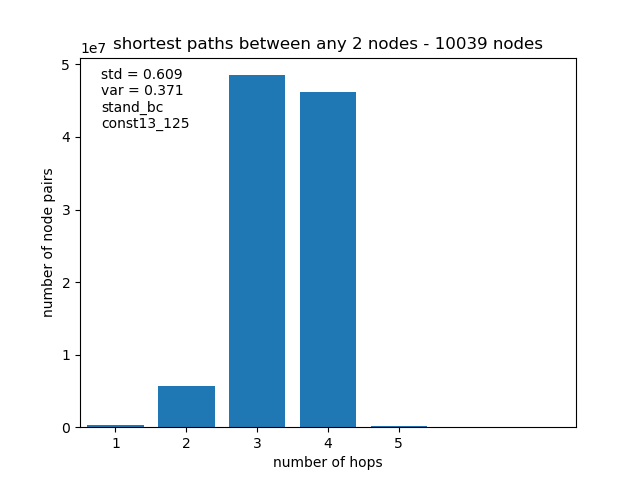
\includegraphics[width=.8\columnwidth]{figures/initConnectDistribution/const13/final-shortest-paths-between-any-nodes-10039-nodes.png}
    \caption{Shortest paths between any two nodes using the standard Bitcoin implementation with 13 initial connections.}
    \label{fig:initConnectDistributionConst13ShortestPath}
\end{figure}

\subsection{Corrupt nodes}

In this subsection we present the results if $1\%$ of the nodes are ``corrupt`` and connect to many more nodes than those initial 8 connections, illustrated in Figures [~\ref{fig:initConnectDistribution1percentAverage},~\ref{fig:initConnectDistribution1percentDegree},~\ref{fig:initConnectDistribution1percentShortestPath}].
The peak of the average hops between one node and all other nodes in Figure [~\ref{fig:initConnectDistribution1percentAverage}] decreases compared to the standard Bitcoin implementation in Figure [~\ref{fig:standardBitcoinAverageHops}]. However, the variance and standard deviation increase.
The behaviour of the corrupt nodes can also be seen very nicely in the degree plot in Figure [~\ref{fig:initConnectDistribution1percentDegree}] where some nodes have very high degrees. Some of them connect to over $10\%$ of the whole network. These corrupt nodes seems to decrease the number of shortest paths in Figure [~\ref{fig:initConnectDistribution1percentShortestPath}] and the number of shortest paths peaks at 3 hops but many nodes can be reached by just 2 hops. The 4 hops that represented the peak in the standard Bitcoin implementation [~\ref{fig:standardBitcoinShortestPaths}] don't play such a big role anymore if $1\%$ of the nodes act as corrupt nodes.

\begin{figure}
    \centering
    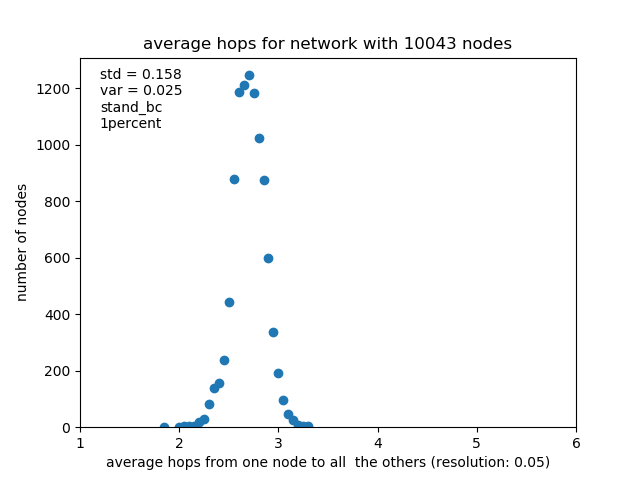
\includegraphics[width=.8\columnwidth]{figures/initConnectDistribution/1percent/average-hops-for-network-with-10043-nodes.png}
    \caption{Average hops from one node to all other nodes using the standard Bitcoin implementation with $1\%$ of the nodes trying to connect to as many other nodes as possible.}
    \label{fig:initConnectDistribution1percentAverage}
\end{figure}

\begin{figure}
    \centering
    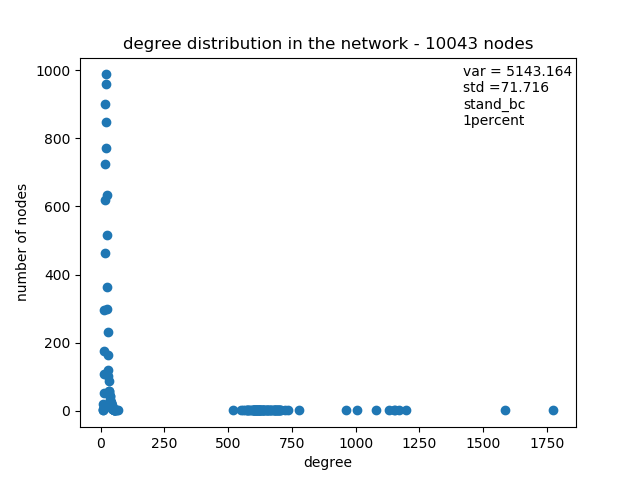
\includegraphics[width=.8\columnwidth]{figures/initConnectDistribution/1percent/degree-distribution-10043-nodes.png}
    \caption{Degree distribution using the standard Bitcoin implementation with $1\%$ of the nodes trying to connect to as many other nodes as possible.}
    \label{fig:initConnectDistribution1percentDegree}
\end{figure}

\begin{figure}
    \centering
    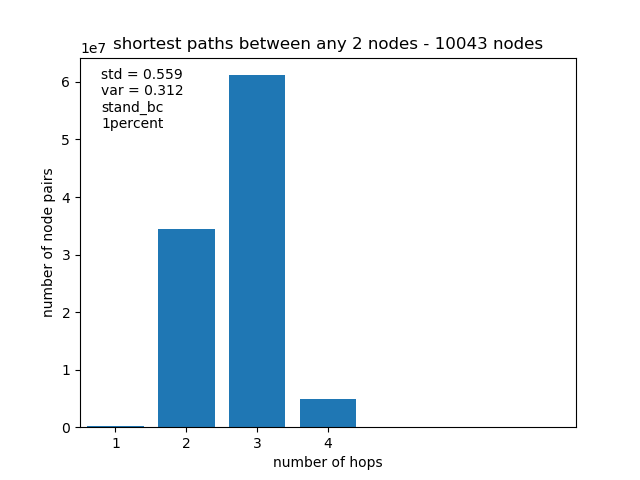
\includegraphics[width=.8\columnwidth]{figures/initConnectDistribution/1percent/final-shortest-paths-between-any-nodes-10043-nodes.png}
    \caption{Shortest paths between any two nodes using the standard Bitcoin implementation with $1\%$ of the nodes trying to connect to as many other nodes as possible.}
    \label{fig:initConnectDistribution1percentShortestPath}
\end{figure}

\section{Power of Two Choices}

The power of two choices minimum implementation results in a slightly higher peak (4.125 hops) in the average path distance as illustrated in Figure [~\ref{fig:p2cMinAverageHops}] compared to the standard Bitcoin implementation in Figure [~\ref{fig:standardBitcoinAverageHops}]. The power of two choices also has a smaller standard deviation and variance as the standard Bitcoin implementation.
Looking at the same plot using the power of two choices maximum algorithm as illustrated in Figure [~\ref{fig:p2cMaxAverageHops}] a smaller peak (3.75 hops) can be noticed compared to the power of two choices minimum algorithm and the standard Bitcoin implementation. However, the standard deviation and variance is bigger for the power of two choices maximum algorithm than the two other implementations.

\begin{figure}
    \centering
    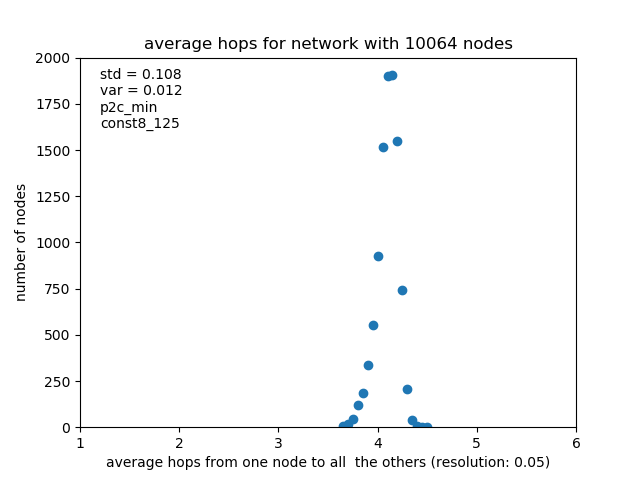
\includegraphics[width=.8\columnwidth]{figures/power2choices/p2c-min/average-hops-for-network-with-10064-nodes.png}
    \caption{The average path distance from one node to any other nodes using the power of two choices minimum approach described in algorithm [~\ref{alg:power2choicesMin}].}
    \label{fig:p2cMinAverageHops}
\end{figure}

\begin{figure}
    \centering
    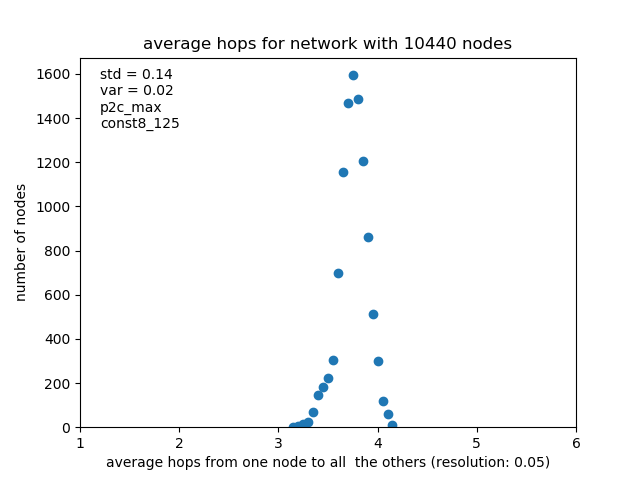
\includegraphics[width=.8\columnwidth]{figures/power2choices/p2c-max/average-hops-for-network-with-10440-nodes.png}
    \caption{The average path distance from one node to any other nodes using the power of two choices maximum approach described in algorithm [~\ref{alg:power2choicesMax}].}
    \label{fig:p2cMaxAverageHops}
\end{figure}

Looking at the degree distribution of the power of two choices minimum algorithm in Figure [~\ref{fig:p2cMinDegree}] and the degree distribution of the power of two choices maximum algorithm in Figure [~\ref{fig:p2cMaxDegree}] there is a clear difference. In the power of two choices minimum algorithm most of the nodes have similar numbers of degree. The degree numbers are even closer together than in the standard Bitcoin implementation [~\ref{fig:standardBitcoinDegree}]. However, in the power of two choices maximum algorithm the degrees are more widely spread over a greater distance. There are nodes with over 60 connections and some have only 8.

\begin{figure}
    \centering
    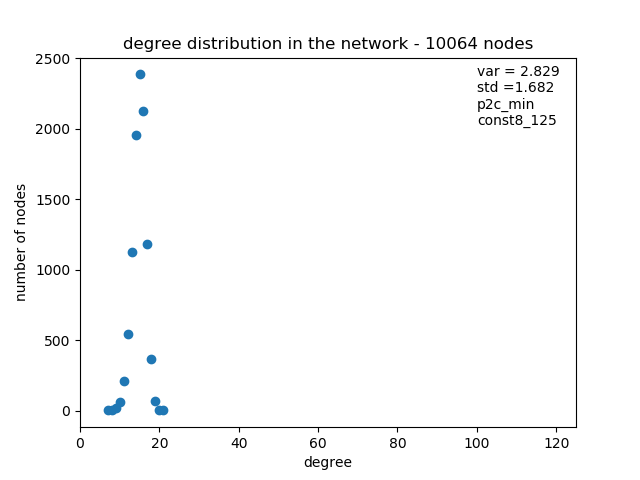
\includegraphics[width=.8\columnwidth]{figures/power2choices/p2c-min/degree-distribution-10064-nodes.png}
    \caption{The degree distribution using the power of two choices minimum approach described in algorithm [~\ref{alg:power2choicesMin}].}
    \label{fig:p2cMinDegree}
\end{figure}

\begin{figure}
    \centering
    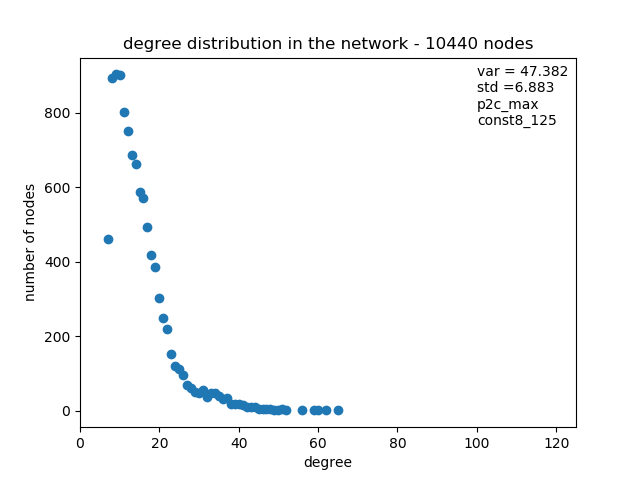
\includegraphics[width=.8\columnwidth]{figures/power2choices/p2c-max/degree-distribution-10440-nodes.png}
    \caption{The degree distribution using the power of two choices maximum approach described in algorithm [~\ref{alg:power2choicesMax}].}
    \label{fig:p2cMaxDegree}
\end{figure}

The shortest paths between any two nodes using the power of two choices minimum algorithm as shown in Figure [~\ref{fig:p2cMinShortestPath}] leads to a result where most node pairs have a distance of 4 hops as in the standard Bitcoin implementation, illustrated in Figure [~\ref{fig:standardBitcoinShortestPaths}]. However, there are more pairs that have a distance of 5 hops than in the standard Bitcoin implementation.
Looking at the shortest paths between any two nodes using the power of two choices maximum algorithm as illustrated in Figure [~\ref{fig:p2cMaxShortestPath}] leads to a result where most pairs take 4 hops to be reached. There are also many node pairs that can be reached in 3 hops. The 5 hops connections are fewer than in the power of two choices minimum algorithm.

\begin{figure}
    \centering
    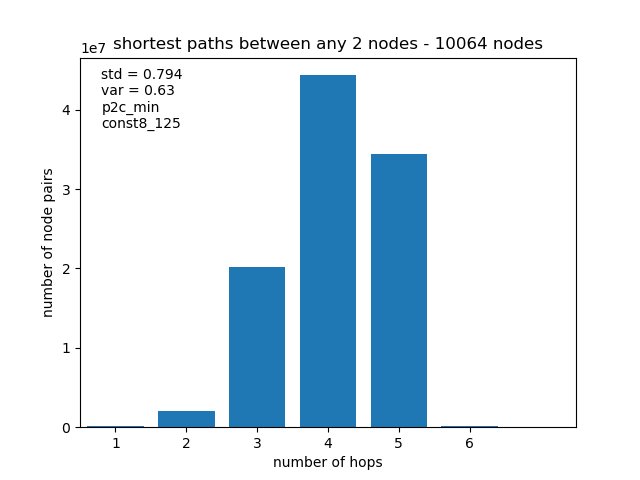
\includegraphics[width=.8\columnwidth]{figures/power2choices/p2c-min/final-shortest-paths-between-any-nodes-10064-nodes.png}
    \caption{The shortest paths between any two nodes using the power of two choices minimum approach described in algorithm [~\ref{alg:power2choicesMin}].}
    \label{fig:p2cMinShortestPath}
\end{figure}

\begin{figure}
    \centering
    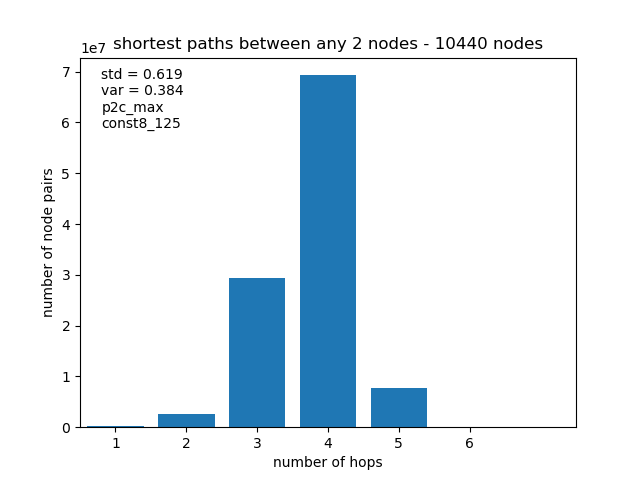
\includegraphics[width=.8\columnwidth]{figures/power2choices/p2c-max/final-shortest-paths-between-any-nodes-10440-nodes.png}
    \caption{The shortest paths between any two nodes using the power of two choices maximum approach described in algorithm [~\ref{alg:power2choicesMax}].}
    \label{fig:p2cMaxShortestPath}
\end{figure}

\section{IP Location Clustering}
If very strict boundaries are set for the propagation delays between two different clusters and within a single cluster the impact of local and inter-cluster connections can be illustrated best. (Using $10ms$ as a propagation delay within the same cluster and $300ms$ as a propagation delay between two different clusters.) In Figures [~\ref{fig:geoCluster-tConst10-300-geo-shortest-path},~\ref{fig:geoCluster-tConst10-300-noGeo-shortest-path}] most nodes within the same cluster are reachable within the first $90ms$ (3 hops inside the own cluster). Most nodes that are located in a different cluster are reachable after $320ms$ (first hop to other cluster and 3 to 4 hops within that cluster or first hop within the same cluster, second hop to other cluster and 3 hops within that other cluster).

\begin{figure}
    \centering
    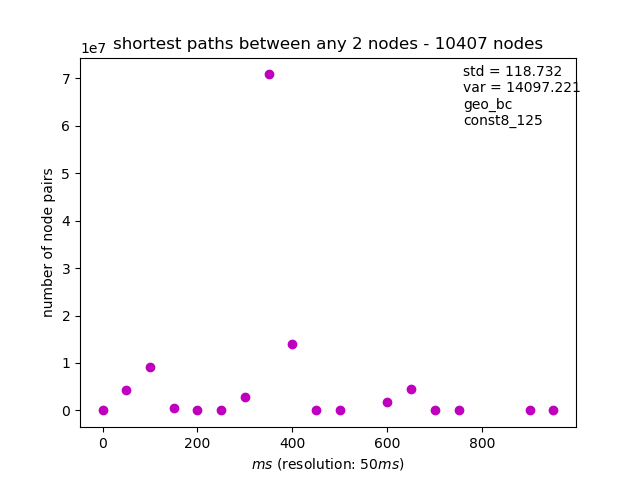
\includegraphics[width=.8\columnwidth]{figures/geoCluster/tConst10-300/geo/final-shortest-paths-between-any-nodes-10407-nodes.png}
    \caption{Shortest paths propagation delay for any node pair with constant propagation delays within the same cluster of $10ms$ and between two different clusters of $300ms$. Clustering as in [~\ref{alg:geo3to5}].}
    \label{fig:geoCluster-tConst10-300-geo-shortest-path}
\end{figure}

\begin{figure}
    \centering
    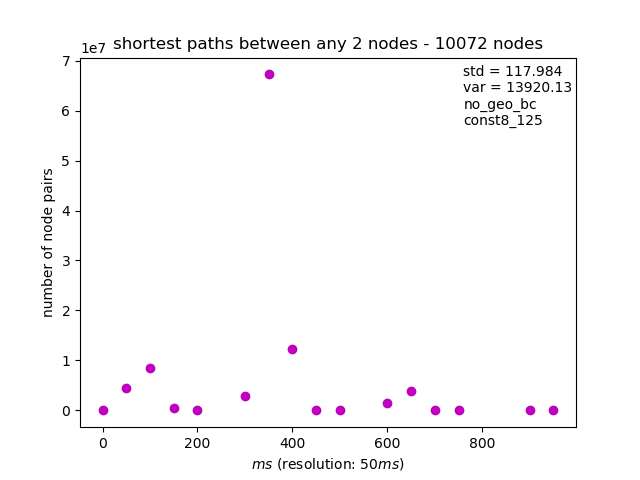
\includegraphics[width=.8\columnwidth]{figures/geoCluster/tConst10-300/noGeo/final-shortest-paths-between-any-nodes-10072-nodes.png}
    \caption{Shortest paths propagation delay for any node pair with constant propagation delays within the same cluster of $10ms$ and between two different clusters of $300ms$. No Clustering.}
    \label{fig:geoCluster-tConst10-300-noGeo-shortest-path}
\end{figure}

Using more realistic values instead of these constant thresholds, a more realistic real world scenario can be simulated. For the propagation delays between different clusters the values in table [~\ref{table:propagationDelayInternational}] have been used as means in a normal distribution with a $\sigma = 10ms$. The propagation delays within the same cluster have been modeled as a normal distribution of $\mu = 30ms$ and $\sigma = 9ms$. These propagation delays are approximated using measurements from wondernetwork~\cite{pingLookup}.
The results of that simulation are illustrated in Figures [~\ref{fig:geoCluster-const8_125-geo-shortest-path},~\ref{fig:geoCluster-const8_125-noGeo-shortest-path}]. Both of the plots look Gaussian too but there is a ``bump`` at $350ms$ just before it peaks at $400ms$. Additionally, both Figures [~\ref{fig:geoCluster-const8_125-geo-shortest-path},~\ref{fig:geoCluster-const8_125-noGeo-shortest-path}] tend to have the same behaviour for using a geographical clustering or not using one at all.

\begin{table}
  \centering
  \begin{tabular}{ | l || c | c | c | c | c | c | }
    \hline
    cities & Cape Town & San Francisco & Sao Paulo & Sydney & Tokyo & Zurich \\ \hline \hline
    Cape Town & - & $298ms$ & $341ms$ & $420ms$ & $377ms$ & $161ms$ \\ \hline
    San Francisco & $298ms$ & - & $171ms$ & $155ms$ & $109ms$ & $176ms$ \\ \hline
    Sao Paulo & $341ms$ & $172ms$ & - & $367ms$ & $269ms$ & $234ms$ \\ \hline
    Sydney & $420ms$ & $155ms$ & $367ms$ & - & $115ms$ & $306ms$ \\ \hline
    Tokyo & $377ms$ & $109ms$ & $269ms$ & $114ms$ & - & $282ms$ \\ \hline
    Zurich & $161ms$ & $176ms$ & $236ms$ & $306ms$ & $281ms$ & - \\ \hline
  \end{tabular}
  
  \caption{This table represents the propagation delays between two cities (which were used as reference cities for their continent) and has been measured by wondernetwork~\cite{pingLookup}.} \label{table:propagationDelayInternational}
\end{table}

\begin{figure}
    \centering
    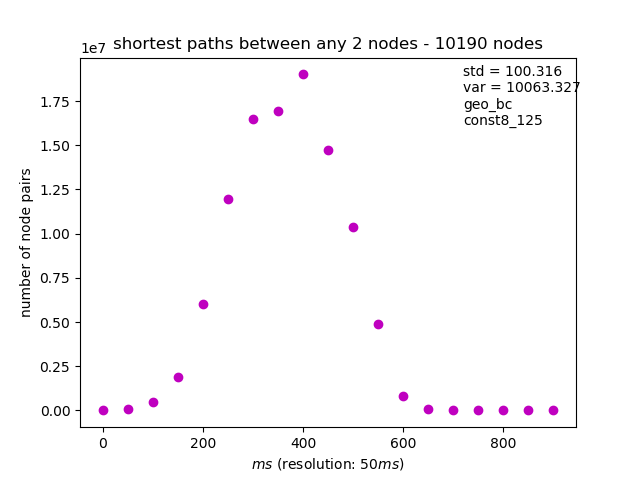
\includegraphics[width=.8\columnwidth]{figures/geoCluster/const8_125/geo/final-shortest-paths-between-any-nodes-10190-nodes.png}
    \caption{Propagation delay between any two nodes with propagation delays from a normal distribution. Clustering as in [~\ref{alg:geo3to5}].}
    \label{fig:geoCluster-const8_125-geo-shortest-path}
\end{figure}

\begin{figure}
    \centering
    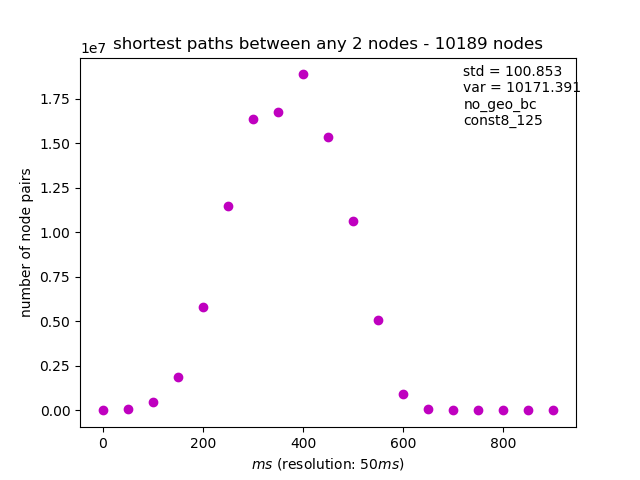
\includegraphics[width=.8\columnwidth]{figures/geoCluster/const8_125/noGeo/final-shortest-paths-between-any-nodes-10189-nodes.png}
    \caption{Propagation delay between any two nodes with propagation delays from a normal distribution. No clustering.}
    \label{fig:geoCluster-const8_125-noGeo-shortest-path}
\end{figure}

In Figure [~\ref{fig:geoCluster-const8_125-geo-average-hops},~\ref{fig:geoCluster-const8_125-noGeo-average-hops}] the average propagation delay from one node to all its other nodes is illustrated.
The use of more realistic propagation delays leads to a distribution that could be approximated by a normal distribution. There is a ``bump`` around $400ms$ until there is another cut-off shortly before $450ms$. However, the use of a geographical clustering versus no geographical mapping does not have a big impact on the average propagation delay.

\begin{figure}
    \centering
    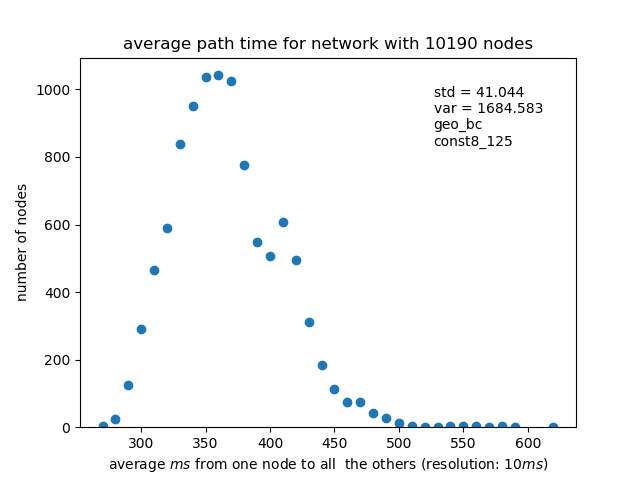
\includegraphics[width=.8\columnwidth]{figures/geoCluster/const8_125/geo/average-hops-for-network-with-10190-nodes.png}
    \caption{Average propagation delay for any node with propagation delays from a normal distribution. Clustering as in [~\ref{alg:geo3to5}].}
    \label{fig:geoCluster-const8_125-geo-average-hops}
\end{figure}

\begin{figure}
    \centering
    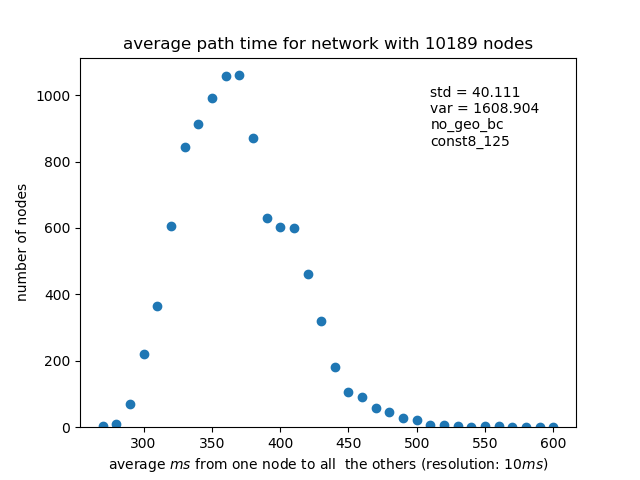
\includegraphics[width=.8\columnwidth]{figures/geoCluster/const8_125/noGeo/average-hops-for-network-with-10189-nodes.png}
    \caption{Average propagation delay for any node with propagation delays from a normal distribution. No clustering.}
    \label{fig:geoCluster-const8_125-noGeo-average-hops}
\end{figure}

A third analysis of the IP clustering looks at what happens if one takes an algorithm with 8 connections inside the same cluster and 5 connections to other clusters. As illustrated in Figures [~\ref{fig:geoCluster-const13_125-geo-shortest-path},~\ref{fig:geoCluster-const13_125-noGeo-shortest-path}] this leads to a faster gossiping of information between nodes compared to the Figures [~\ref{fig:geoCluster-const8_125-geo-shortest-path},~\ref{fig:geoCluster-const8_125-noGeo-shortest-path}]. However, the difference between the use of the standard Bitcoin implementation and the implementation with the geographical clustering is minor. In both of them one sees a distribution with two peaks (at $250ms$ and at $350ms$).

\begin{figure}
    \centering
    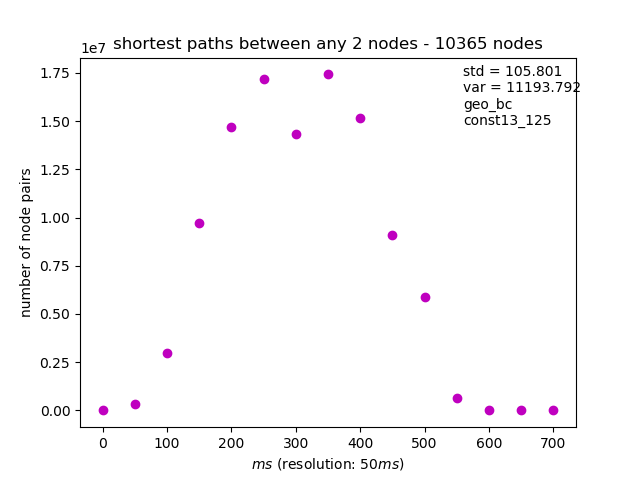
\includegraphics[width=.8\columnwidth]{figures/geoCluster/const13_125/geo/final-shortest-paths-between-any-nodes-10365-nodes.png}
    \caption{Shortest path propagation delay for all node pairs with propagation delays from a normal distribution. Clustering as in [~\ref{alg:geo8to5}].}
    \label{fig:geoCluster-const13_125-geo-shortest-path}
\end{figure}

\begin{figure}
    \centering
    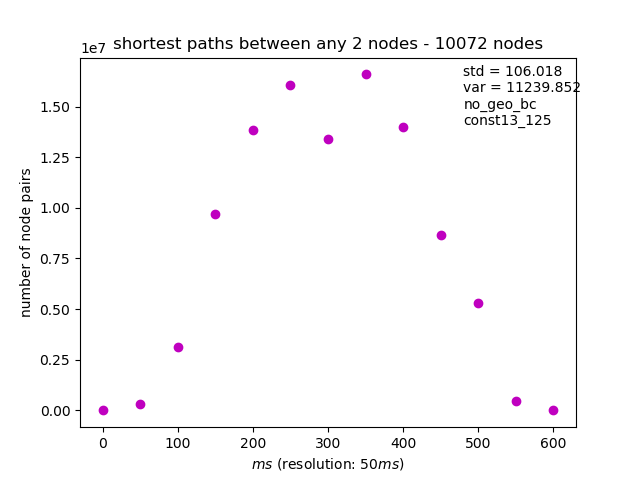
\includegraphics[width=.8\columnwidth]{figures/geoCluster/const13_125/noGeo/final-shortest-paths-between-any-nodes-10072-nodes.png}
    \caption{Shortest path propagation delay for all node pairs with propagation delays from a normal distribution. No clustering.}
    \label{fig:geoCluster-const13_125-noGeo-shortest-path}
\end{figure}

\chapter{Discussion of Result}

\section{Influence of Initial Connections}

The standard Bitcoin implementation of the connection strategy seems to be a reliable way to connect single Bitcoin nodes in an efficient way as the figures [~\ref{fig:standardBitcoinAverageHops},~\ref{fig:standardBitcoinDegree},~\ref{fig:standardBitcoinShortestPaths}] demonstrate.
As Miller et al. ~\cite{DiscoveringBitcoinsPublicTopologyAndInfluentialNodes} showed, there are in practice some influential nodes that don't follow the standard implementation and try to connect to many more nodes. Eyal et al.~\cite{MajorityIsNotEnough} claim that if a node manages to spread its information more quickly than other nodes and get other information more quickly as a result too, it could gain advantage from deviating from the protocol.
In the simulation of [~\ref{fig:initConnectDistribution1percentAverage},~\ref{fig:initConnectDistribution1percentDegree},~\ref{fig:initConnectDistribution1percentShortestPath}] where this situation is created artificially, we claim that having a few nodes that are highly connected (very high degree) leads to a network that has much shorter minimal paths between two different nodes. This result is expected since as soon as the message arrives at a highly connected node it can be distributed to many more nodes than usual which leads to a decrease in shortest paths especially if there are multiple such highly connected nodes.
This indicates that these influential nodes are actually beneficial to decrease the number of hops a message has to take on average to reach all nodes.

To decrease the number of hops we also tried a brute-force method. We increased the number of initial connections as the Figures [~\ref{fig:initConnectDistribution8variation-big},~\ref{fig:initConnectDistribution8variation-small}] illustrate. The decrease of average hops can be explained with every single node having a higher degree which makes the network more connected. The flattening of the curve at 2.5 hops after approximately 48 initial connections could be explained that there is a limit at 1 anyway (every node connects to every other node) but for every slight improvement of the average hops there need to be many more edges implemented after this flattening region.

This brute-force method can be analyzed in more detail with the example of 13 initial connections as demonstrated in Figures [~\ref{fig:initConnectDistributionConst13Average},~\ref{fig:initConnectDistributionConst13Degree},~\ref{fig:initConnectDistributionConst13ShortestPath}]. The decrease of the standard deviation, variance and number of hops for all shortest paths results in more fairness because all nodes get the same information more synchronized (lower variance of the hops) as well as more speed because the average number of hops there have to be taken decreases.
However, the bottleneck of this implementation is the available bandwidth of each individual node.
Some nodes have due to their infrastructure no problem allocating more bandwidth to their Bitcoin system. Hence, it could be reasonable to make the current 8 initial nodes a bit more flexible and allow by default nodes with better connections to have up to 13 initial connections because of the benefit in fairness and speed it would give the whole network.

\section{Power of Two Choices}

The power of two choices algorithm assumes that if one asks a neighbour about the degree of its connectivity that he is not going to lie in order to profit from the protocol. This assumption can be made since most Bitcoin nodes are simply running the standard Bitcoin implementation and would therefore not lie.

The power of two choices minimum algorithm leads to a balancing of the degrees where most nodes have roughly the same degree (can be seen in figure [~\ref{fig:p2cMinDegree}]) which matches the theoretical concept that Mitzenmacher et al. ~\cite{Power2Choices} have proven.
A nice side effect of this behaviour is that it also lowers the standard deviation and variance of the average path length of one node to any other node as seen in figure [~\ref{fig:p2cMinAverageHops}]. This leads to an increase in fairness within the network since on average nodes receive information more synchronized. However, there is a cost to this strategy as well; on average the shortest path between two nodes is longer than in the standard Bitcoin implementation.

The power of two choices maximum algorithm on the other hand improves the average of the shortest paths between any two nodes as seen in figure [~\ref{fig:p2cMaxAverageHops}] but the standard deviation and variance is larger than the standard Bitcoin implementation which leads to greater speed but less fairness.

Each one of the two algorithms are only able to improve one metric but get worse on the other.
There seems to be a pay off between having some nodes that have higher degree and are therefore able to spread information in fewer hops on average leading to an increase of speed and having more balanced degrees that lead to a smaller standard deviation and variance of the average hops for each node and therefore fairness increases.

\section{IP Location Clustering}

The IP Location Clustering algorithm is a different approach that utilizes the knowledge of the physical topology. As illustrated in the Figures [~\ref{fig:geoCluster-const8_125-geo-shortest-path}, ~\ref{fig:geoCluster-const8_125-noGeo-shortest-path}, ~\ref{fig:geoCluster-const8_125-geo-average-hops}, ~\ref{fig:geoCluster-const8_125-noGeo-average-hops}, ~\ref{fig:geoCluster-const13_125-geo-shortest-path}, ~\ref{fig:geoCluster-const13_125-geo-shortest-path}, ~\ref{fig:geoCluster-const13_125-noGeo-shortest-path}] one can not see much of a difference between the use of geographical information compared to not using geographical information at all.

However, since it has the potential to perform equally well compared to the standard Bitcoin implementation it might be an alternative way to set up the network.

\chapter{Conclusion}

Although a ground-breaking algorithm that dramatically improves the bitcoin network topology seems a difficult task, in this work we explored multiple strategies and gained valuable insight on how the connection strategy in Bitcoin works and what happens if certain parameters are being changed.
However, we were able to show that on average highly connected nodes lead to a decrease of hops for messages to be passed from one node to its destination node. Additionally, we were able to show that a brute-force approach (increasing the initial connections) leads on average to a faster message passing between node pairs, as expected. This brute force approach also leads to a greater fairness because the standard distribution of the shortest paths decreases. 

The power of two choices is a simple and elegant approach. The power of two choices minimum algorithm improves the fairness but lowers the speed. That is because all nodes end up having roughly the same degree which leads to shortest path lengths that show a smaller standard deviation.
The power of two choices maximum algorithm does the opposite. It creates nodes that have a higher degree and therefore increase the standard deviation from the shortest path lengths but at the same time decreases those path lengths on average.
Therefore, the power of two choices protocol might be of some use if an algorithm has to be designed that only needs to improve either-one of these metrics.

The IP Location Clustering idea shows a similar behaviour as the current standard Bitcoin implementation. It could therefore be used as an alternative to the current standard Bitcoin protocol.

Concluding, a bigger use of bandwidth (more edges in the network) of individual nodes is so far the simplest approach to decrease hops and increase the networks fairness and speed.

% This displays the bibliography for all cited external documents. All references have to be defined in the file references.bib and can then be cited from within this document.
\bibliographystyle{IEEEtran}
\bibliography{references}

% This creates an appendix chapter, comment if not needed.
%\appendix
%\chapter{Algorithms}

\end{document}